\documentclass[12pt]{article} 
\usepackage{pythonhighlight}

\usepackage[utf8]{inputenc}

% font types
\renewcommand{\familydefault}{\sfdefault}
% \usepackage{helvet}
% \usepackage[T1]{fontenc}
% \usepackage[utf8]{inputenc}

% package to rotate the page landscape 
%\usepackage[paper=portrait, pagesize]{typearea}
\usepackage[a4paper]{geometry}
\usepackage[usegeometry]{typearea}
%\usepackage[hmargin=.65in,vmargin=1.1in]{geometry}
%\usepackage[top=0.75in, left=0.75in, right=0.52in, bottom=1.44in]{geometry}

% only for dummy text
\usepackage{blindtext}
\usepackage{lipsum}
%\usepackage[margin=0.5in, left=0.5in, top=0.8in, includefoot]{geometry}
%\usepackage[a4paper, left=1.0in, right=1.0in, top=1.0in, bottom=1.0in]{geometry}

\usepackage[hidelinks]{hyperref} % Allows for clickable references

% Graphics preamble
\usepackage{graphicx} % import graphics package
%\graphicspath{ {/Users/tgol0003/Desktop/seagate4_2/uwgeo_models/production_models/} } % harddisk path
\usepackage{float} % Allows for control of float positions
\usepackage[section]{placeins} % to place figures in the section 
\usepackage{multicol} % position figures across the columns

% figures packages

% adding number with in section to equations
\usepackage{amsmath} 
\numberwithin{equation}{subsection} 
\makeatletter
\@addtoreset{equation}{section}
\makeatother

% Header and Footer info
\usepackage{fancyhdr}
\pagestyle{fancy}
\fancyhead{}
\fancyfoot{}
\fancyfoot[R]{\thepage}
\renewcommand{\headrulewidth}{0pt}
\renewcommand{\footrulewidth}{0pt}

\newgeometry{left=0.35in, right=0.35in, top=0.5in, bottom=1.0in}

\usepackage{changepage}

\begin{document} 

\cleardoublepage
\KOMAoptions{paper=portrait}
\recalctypearea
\newgeometry{left=0.1in, right=0.1in, top=0.1in, bottom=0.1in}


%\eject \pdfpagewidth=8.3in \pdfpageheight=11.7in % a4 dim


	
\begin{figure*}
	\vspace{-1.2in}
	\begin{multicols}{1}
		\hspace{3.65in} 
\includegraphics[width=2cm]{../Annulus_Benchmark_Kramer/benchmark_figs/label_Free-Slip.pdf}
	\end{multicols}
	
	\vspace{-0.3in}
		
	\begin{multicols}{3}
		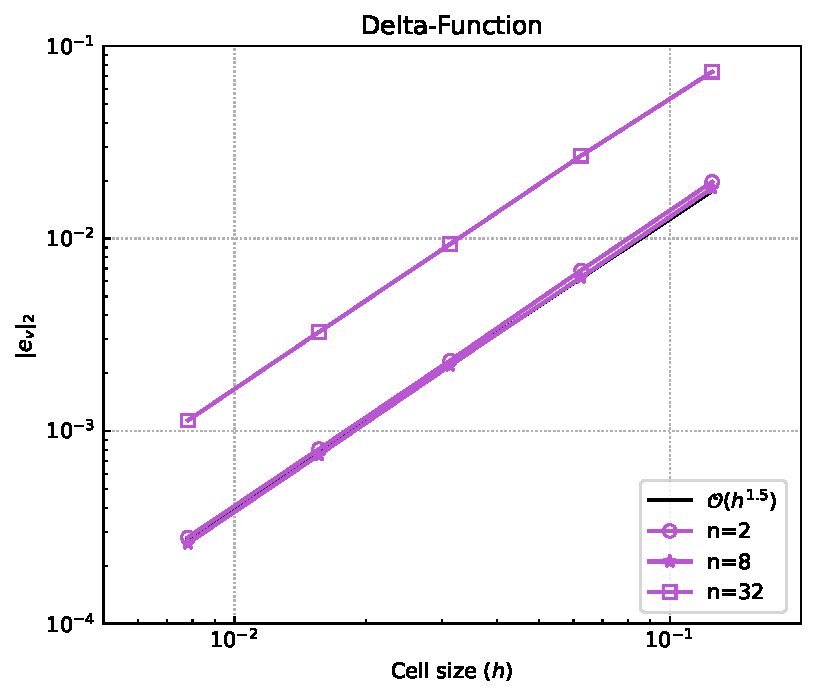
\includegraphics[width=6.85cm]{../Annulus_Benchmark_Kramer/benchmark_figs/case1_k_0_vel_err_conv_vel_penalty_2.5e+08_stokes_tol_1.0e-10.pdf}\par
		\hspace{-0.08in}
		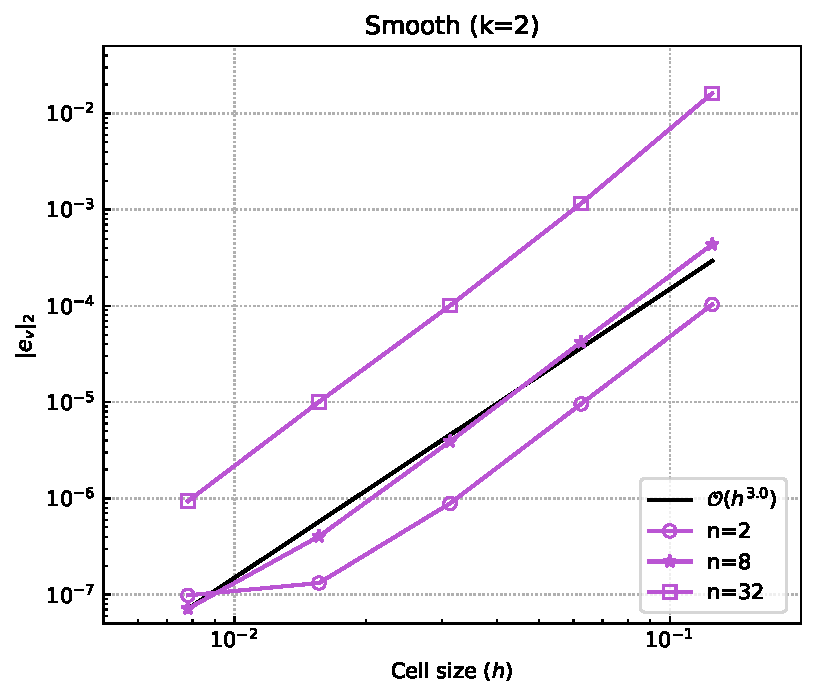
\includegraphics[width=6.85cm]{../Annulus_Benchmark_Kramer/benchmark_figs/case2_k_2_vel_err_conv_vel_penalty_2.5e+08_stokes_tol_1.0e-10.pdf}\par
		\hspace{-0.12in}
		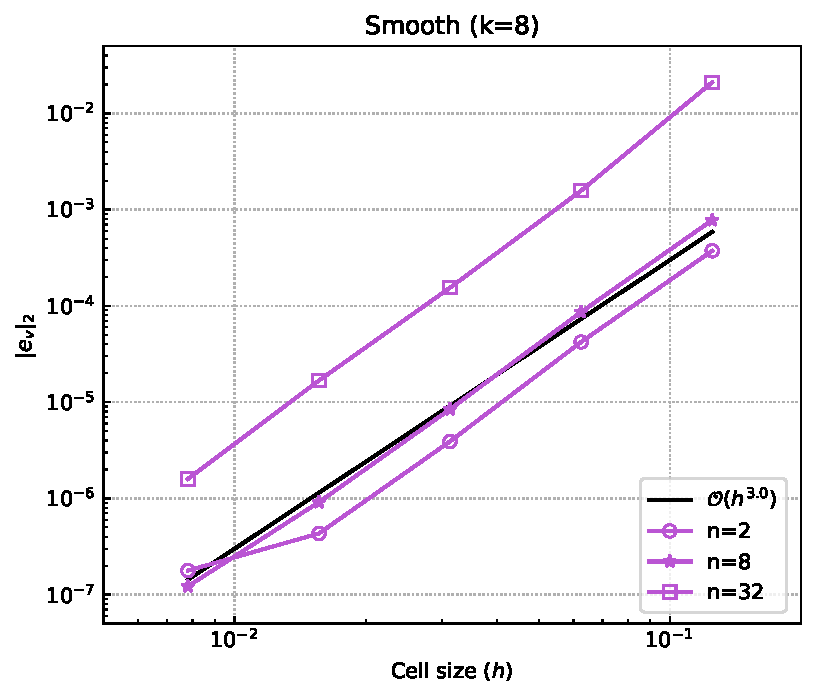
\includegraphics[width=6.85cm]{../Annulus_Benchmark_Kramer/benchmark_figs/case2_k_8_vel_err_conv_vel_penalty_2.5e+08_stokes_tol_1.0e-10.pdf}
	\end{multicols}
	
	\vspace{-0.35in}
	
	\begin{multicols}{3}
	    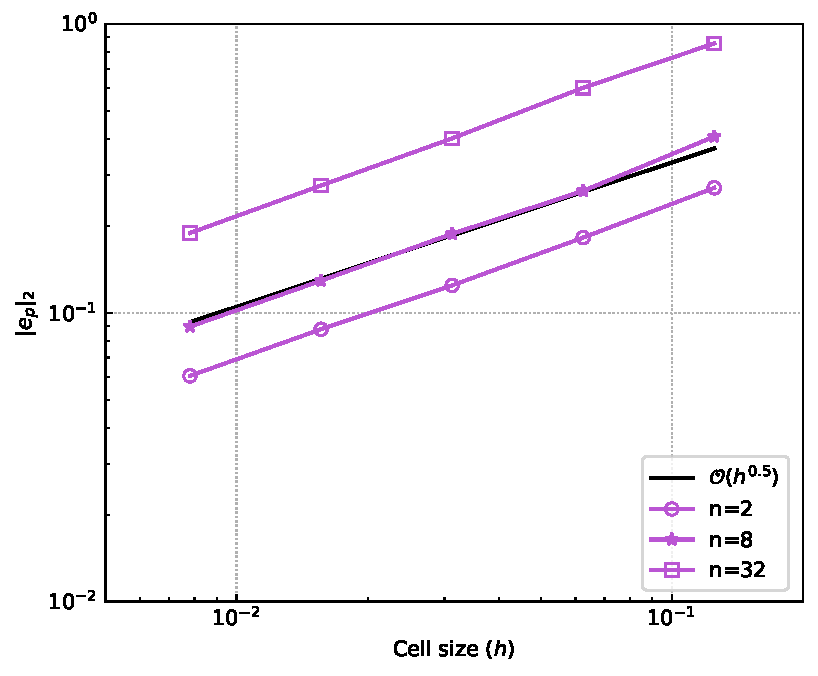
\includegraphics[width=6.85cm]{../Annulus_Benchmark_Kramer/benchmark_figs/case1_k_0_p_err_conv_vel_penalty_2.5e+08_stokes_tol_1.0e-10.pdf}\par
		\hspace{-0.08in} 
		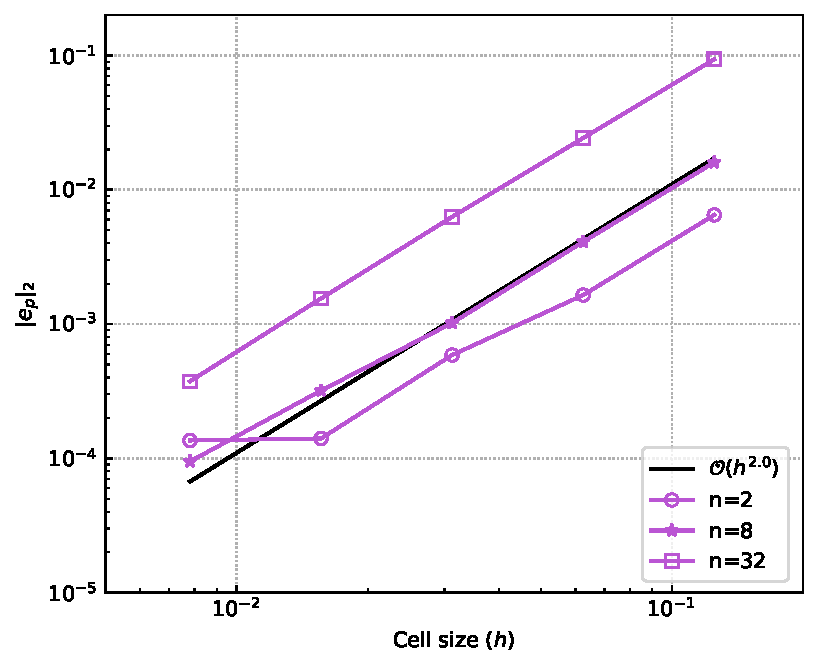
\includegraphics[width=6.85cm]{../Annulus_Benchmark_Kramer/benchmark_figs/case2_k_2_p_err_conv_vel_penalty_2.5e+08_stokes_tol_1.0e-10.pdf}\par
		\hspace{-0.12in}
		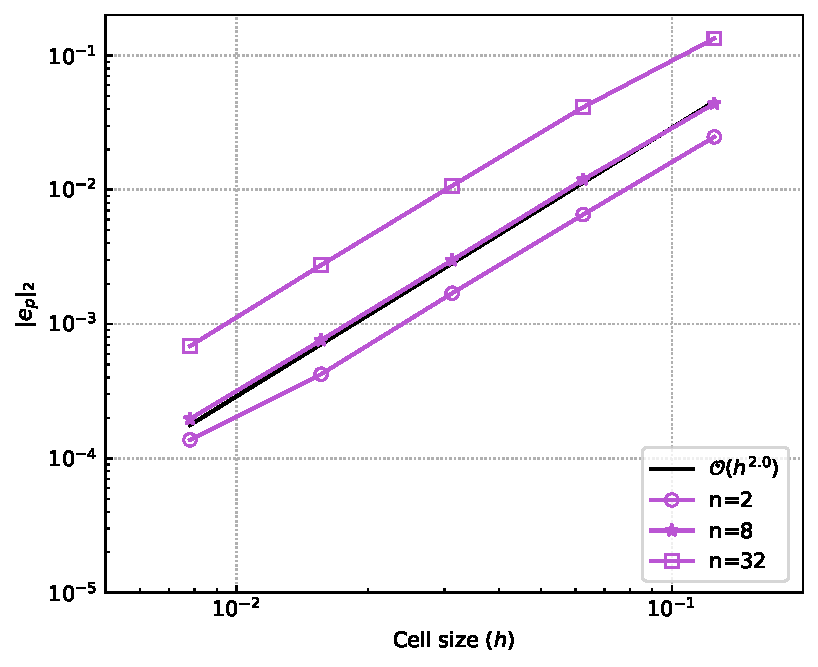
\includegraphics[width=6.85cm]{../Annulus_Benchmark_Kramer/benchmark_figs/case2_k_8_p_err_conv_vel_penalty_2.5e+08_stokes_tol_1.0e-10.pdf}
	\end{multicols}
	
	\vspace{-0.2in}
	\begin{multicols}{1}
		\hspace{3.65in} 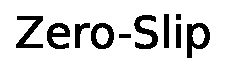
\includegraphics[width=2cm]{../Annulus_Benchmark_Kramer/benchmark_figs/label_Zero-Slip.pdf}
	\end{multicols}
	
	\vspace{-0.3in}
	
	\begin{multicols}{3}
		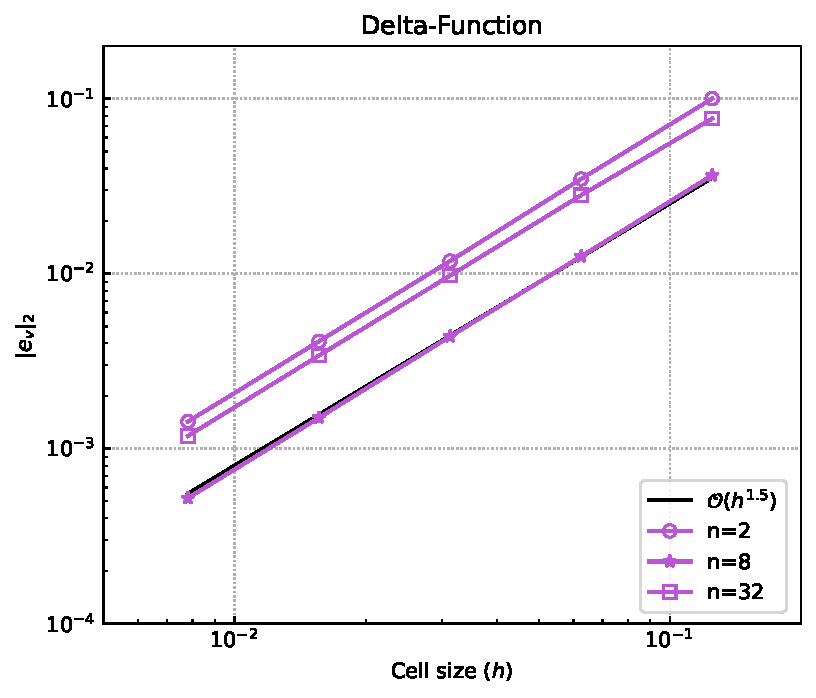
\includegraphics[width=6.85cm]{../Annulus_Benchmark_Kramer/benchmark_figs/case3_k_0_vel_err_conv_vel_penalty_2.5e+08_stokes_tol_1.0e-10.pdf}\par
		\hspace{-0.08in}
		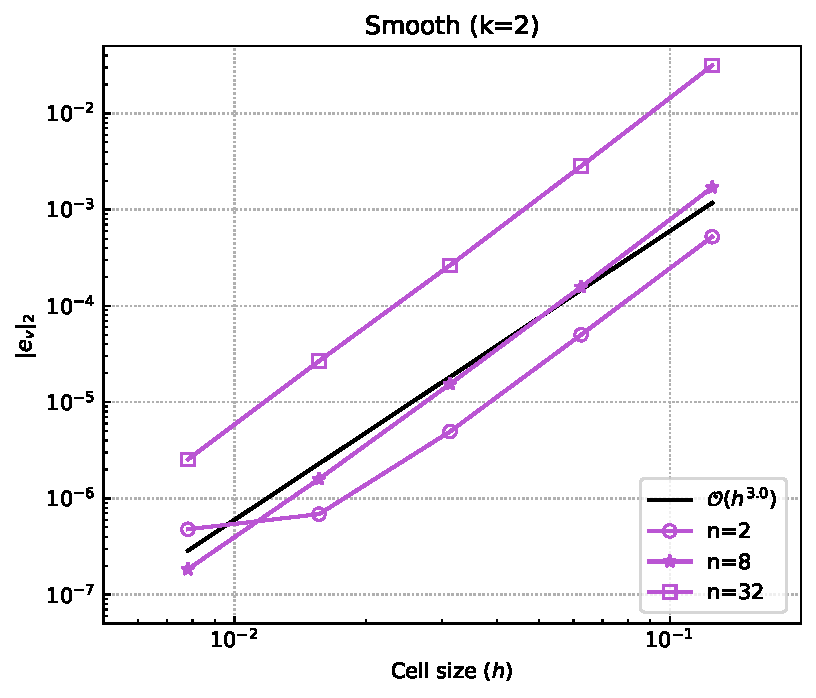
\includegraphics[width=6.85cm]{../Annulus_Benchmark_Kramer/benchmark_figs/case4_k_2_vel_err_conv_vel_penalty_2.5e+08_stokes_tol_1.0e-10.pdf}\par
		\hspace{-0.12in}
		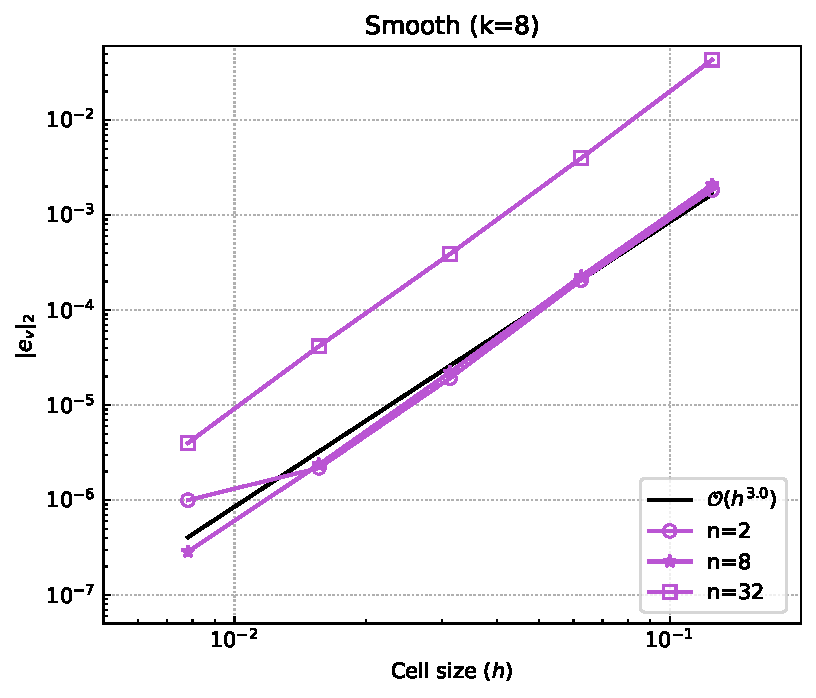
\includegraphics[width=6.85cm]{../Annulus_Benchmark_Kramer/benchmark_figs/case4_k_8_vel_err_conv_vel_penalty_2.5e+08_stokes_tol_1.0e-10.pdf}
	\end{multicols}
	
	\vspace{-0.35in}
	
	\begin{multicols}{3}
		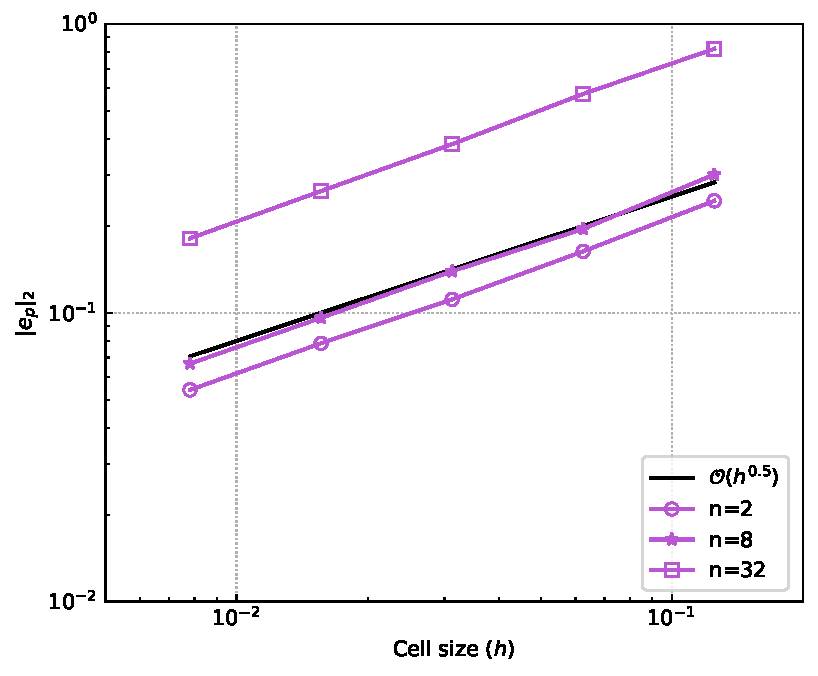
\includegraphics[width=6.85cm]{../Annulus_Benchmark_Kramer/benchmark_figs/case3_k_0_p_err_conv_vel_penalty_2.5e+08_stokes_tol_1.0e-10.pdf}\par
		\hspace{-0.08in} 
		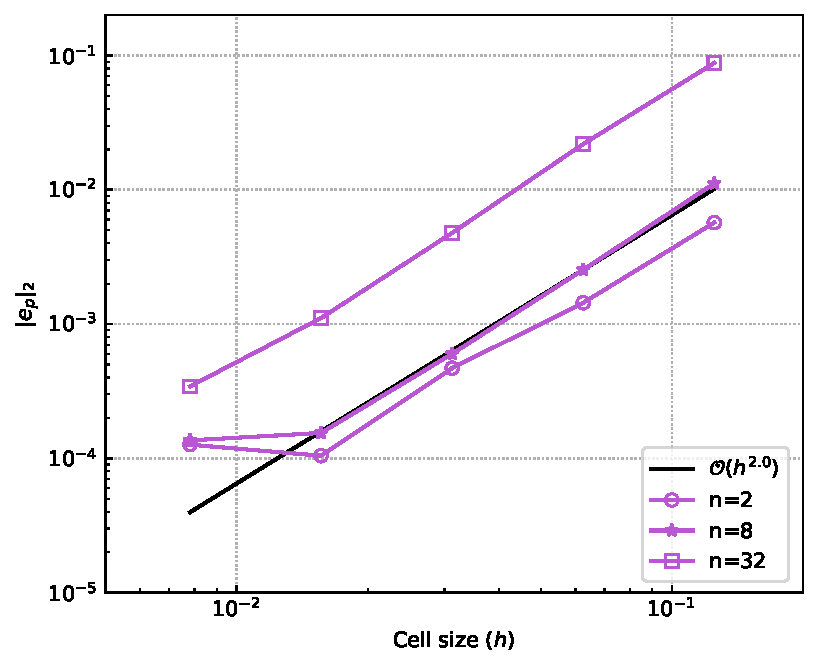
\includegraphics[width=6.85cm]{../Annulus_Benchmark_Kramer/benchmark_figs/case4_k_2_p_err_conv_vel_penalty_2.5e+08_stokes_tol_1.0e-10.pdf}\par
		\hspace{-0.12in}
		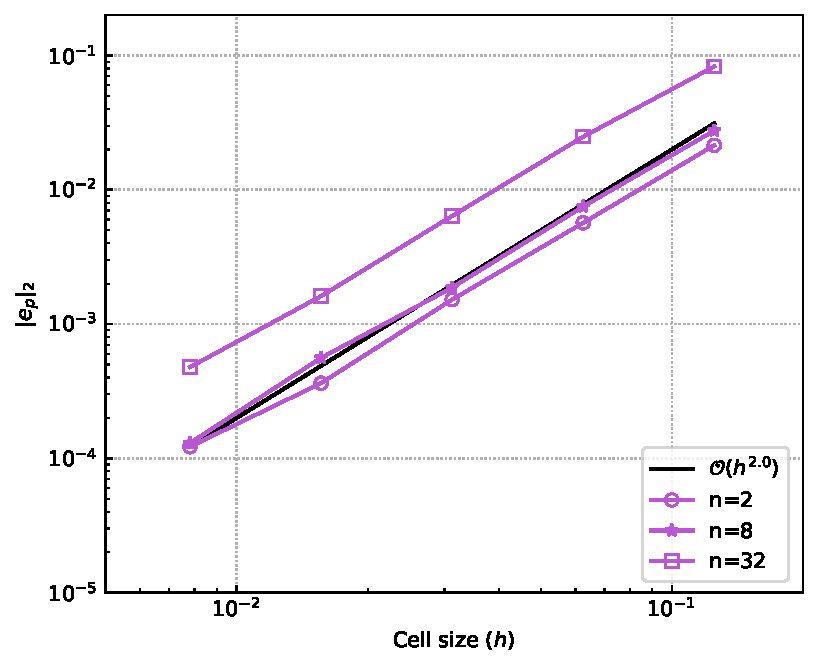
\includegraphics[width=6.85cm]{../Annulus_Benchmark_Kramer/benchmark_figs/case4_k_8_p_err_conv_vel_penalty_2.5e+08_stokes_tol_1.0e-10.pdf}
	\end{multicols}
	
\end{figure*}


\end{document}